\documentclass[11pt,journal]{article}
%\usepackage{hyperref}
%\usepackage[breaklinks]{hyperref}
\usepackage{breakurl}
\usepackage{url}
\usepackage{listings}
\usepackage{courier}
\usepackage{amsmath}
\usepackage{graphicx}
\graphicspath{ {/home/agata/Documents/coursework/SensorNetworks/Project/} }
%\ifCLASSOPTIONcompsoc
% IEEE Computer Society needs nocompress option
% requires cite.sty v4.0 or later (November 2003)
\usepackage[nocompress]{cite}

%\else
% normal IEEE
\usepackage{cite}
%\fi

\hyphenation{op-tical net-works semi-conduc-tor}
\addtolength{\oddsidemargin}{-.875in}
\addtolength{\evensidemargin}{-.875in} 
\addtolength{\textwidth}{1.75in}

\addtolength{\topmargin}{-.875in}
\addtolength{\textheight}{1.75in}

\begin{document}
	\title{Sensor Networks and Mobile Data Communication, Assignment 4}
	
	\author{UID: 1690550}% <-this % stops a space
		%\protect\\
		%\thanks{}}
	
	% The paper headers



	% IEEEtran.cls defaults to using nonbold math in the Abstract.
	% This preserves the distinction between vectors and scalars. However,
	% if the journal you are submitting to favors bold math in the abstract,
	% then you can use LaTeX's standard command \boldmath at the very start
	% of the abstract to achieve this. Many IEEE journals frown on math
	% in the abstract anyway. In particular, the Computer Society does
	% not want either math or citations to appear in the abstract.
	
	% Note that keywords are not normally used for peerreview papers.
	
	% make the title area
	\maketitle
	
	
	% To allow for easy dual compilation without having to reenter the
	% abstract/keywords data, the \IEEEcompsoctitleabstractindextext text will
	% not be used in maketitle, but will appear (i.e., to be "transported")
	% here as \IEEEdisplaynotcompsoctitleabstractindextext when compsoc mode
	% is not selected <OR> if conference mode is selected - because compsoc
	% conference papers position the abstract like regular (non-compsoc)
	% papers do!
	%\IEEEdisplaynotcompsoctitleabstractindextext
	% \IEEEdisplaynotcompsoctitleabstractindextext has no effect when using
	% compsoc under a non-conference mode.
	
	
	% For peer review papers, you can put extra information on the cover
	% page as needed:
	% \ifCLASSOPTIONpeerreview
	% \begin{center} \bfseries EDICS Category: 3-BBND \end{center}
	% \fi
	%
	% For peerreview papers, this IEEEtran command inserts a page break and
	% creates the second title. It will be ignored for other modes.
	%\IEEEpeerreviewmaketitle
	\section{Introduction}
	The simulated problem involves a delay-tolerant network (DTN), with two stationary nodes 0 and 2, positioned 10000 m apart, and a mobile node 1, moving between them. The initial position of the nodes are shown in Fig. 1. We introduce the movement later; for now Node 1 is stationary.
	
	\begin{figure}[h]
		\centering
		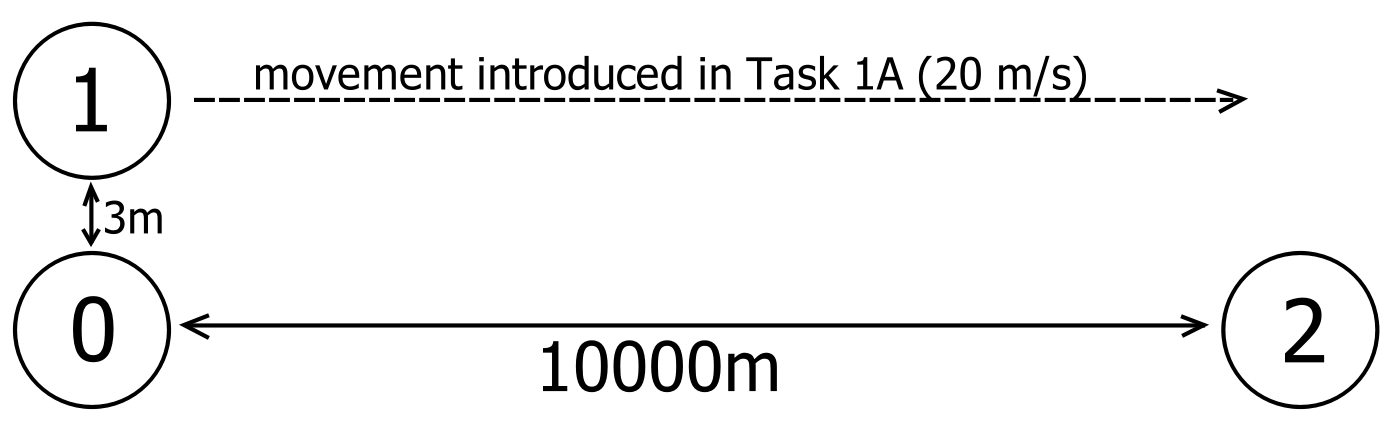
\includegraphics[]{project_topology1.png}
		\caption{Initial topology of the network, with the movement as introduced in the first task}
	\end{figure}

	\subsection{Node 0}
	The code responsible for Node 0 (first village) behaviour starts at line 234 of the original code. 
	
	The function \texttt{Node0DataGen()} maintains the buffer with the messages. It calls itself every second. With each call, it increases the \texttt{global\_counter} variable which acts as a stamp for the mails, and adds the message to the buffer, by updating the head. If adding the message to the buffer would exceed the buffer size, it also moves the tail forward. On the other hand, if the buffer is empty, it also marks the \texttt{isbufferempty} flag as non-empty after adding a message to the buffer. In this case, the tail and head are set to 1.
	
	Sending the messages to Node1 (the bus) is done by \texttt{Node0SendPacket(...)} function. It tries to send the buffer from Node0 every 0.25 seconds. The encapsulation of the buffer is done by creating a \texttt{MyHeader} object. It contains the following pieces of information:
	
	\begin{itemize}
		\item packet type, which here is always 1 for data
		\item \texttt{isbufferempty} - the flag indicating that the buffer is empty. Given that this is performed within an if statement, only if the buffer contains messages, this value should always be 0.
		\item \texttt{head} - head of the buffer
		\item \texttt{tail} - tail of the buffer
	\end{itemize}

	The \texttt{MyHeader} is then put into a packet and sent. If the buffer is empty, instead of creating a \texttt{MyHead} we just log that there is nothing to send.
	
	Finally, whenever Node0 receives an acknowledgement from Node1 that it got the packet with messages, it clears the buffer by setting \texttt{isbufferempty} to 0.
	
	\subsection{Node 1}
	The code describing Node1's behaviour starts at line 298. It has three functions, \texttt{Node1ReceivePacket(...)}, \texttt{Node1AckLoop(...)},and \texttt{Node1SendPacket(...)}. 
	
	The \texttt{Node1ReceivePacket(...)} picks up packets sent by Node0. If it's a data packet, it copies the packet's content into its own buffer, and sets \texttt{Node1SendAck} flag to 1. If it's not a data packet, then it is an acknowledgement from Node 2, which gets logged.
	
	When \texttt{Node1SendAck} flag is set to 1, the \texttt{Node1AckLoop(...)}function, running every 0.01 s, sends the acknowledgement, unsets the \texttt{Node1SendAck} and sets the \texttt{Node1Pending} flag to 1. Finally it schedules the packet to be sent to Node2.
	
	Once the acknowledgement is sent, \texttt{Node1SendPacket(...)} begins its attempts to send the packet to Node2, in 0.25 s intervals. It copies information stored in its buffer to a packet and tries sending it.
	
	\subsection{Node 2}
	
	Node2's role is to receive packets from Node1 and acknowledge it. Starting at line 373, the receiving of packets is covered by function \texttt{Node2ReceivePacket(...)}. It extracts the information from the header and stores them in local variables. Of a particular note is the \texttt{Pkt\_no\_last\_seen\_by\_node2}. It keeps track of the last received packet by storing the stamp of the last message in the previous packet. If the arriving packet contains a message with a newer stamp, Node2 updates its records, and logs the values from the header. Finally it marks \texttt{Node2SendAck}, which will then be used to prompt an acknowledgement.
	
	\texttt{Node2AckLoop(...)} runs at 0.01 s intervals. Every time it creates a packet, however it is sent only if \texttt{Node2SendAck} is marked as 1 by the previous function, after being set to type 0 for ack (cf. 1 for data). This function also logs that the acknowledgement is sent, and marks \texttt{Node2SendAck} back to 0.
	
	\subsection{Overall behaviour}
	
	All nodes are set to unicast mode, with Node0 connected to Node1, and Node1 connected to Node2. They all follow the 802.11 standard, and adhere to AODV protocol with route timeout of 10 min. Note that this is longer than the simulation, which runs for 500 s. The transmission power remains constant at 1.5 dBm throughout the simulation. 
	
	The transmission rate is 2 Mbps. For packets of size 200 bytes, transfer of a single packet would take 0.0008 s, which is barely significant for this simulation.
	
	\subsection{Propagation Loss Model}
	
	The propagation loss model is constant range, which means that up to the given maximum distance (200 m initially) the packets are transmitted with the given transmission power (1.5 dBm in this case). Beyond the maximum range, the transmission power drops to -1000 dBm, which is effectively 0\cite{range loss doc}. Note that with Node1 travelling along the $y=3$ line, it means that it needs to be at $x \leq 199.98 \approx 200$ to reach Node0, and at $ x > 9800$ to reach Node2.
	
	
	
	\begin{thebibliography}{1}
		\bibitem{range loss doc}
		Range Propagation Loss Model, NS-3 documentation, available online: \url{https://www.nsnam.org/doxygen/classns3_1_1_range_propagation_loss_model.html}
	\end{thebibliography}
	% that's all folks
\end{document}

